% Preamble: \usepackage{booktabs,tabularx,graphicx,tikz}
%           \usetikzlibrary{positioning,arrows.meta,calc}
\section{Methodology}
\label{sec:method}

We start from the 731 tasks of SWE-Bench Pro Public v1.0. A task consists of an instruction (problem statement, requirements, new interfaces), a container image with the repository at its base commit, a reference patch, a hidden test patch, fail-to-pass and pass-to-pass lists naming the graded tests, and a verifier that applies the test patch, runs the tests and parses the output. A task is valid if every solution that satisfies the instruction passes and every solution that does not, fails. Figure~\ref{fig:pipeline} traces the tasks through three repair rounds, an engineer review and a final review. Round~1 repaired 40 container images whose reference patches carried test and fixture files or whose instructions lacked the standard template. Round~2 ran an automated audit of difficulty calibration, instruction--test alignment and reward hacking; it flagged 387 tasks (53\%), found 326 clean and errored on 18. Engineers revised the flagged tasks to align instructions with the graded tests and to cover the stated requirements, re-auditing each batch, until about 700 passed; about 30 could not be made to pass through task edits alone. Three changes applied to every task: the \textit{``do not edit tests''} constraint left the instruction template and the verifier now reverts test-related changes before applying the test patch; git history was scrubbed from the images so that agents cannot recover the fix; and network access was disabled in the agent phase, after a frontier model copied reference solutions verbatim from GitHub on 351 solved tasks, only 237 of which held up with GitHub blocked. The result kept all 731 tasks. Round~3 ran two agentic audits (\S\ref{sec:audits}), which flagged 200 tasks (27\%). Engineers adjudicated every flag (\S\ref{sec:review}): 68 tasks were repaired, 43 kept unchanged and 89 discarded. A final review extended task-specific edits across the whole set, and the shared verifier was hardened for every task (\S\ref{sec:verifier}). The release has 642 tasks, 391 of which carry a task-specific repair (Table~\ref{tab:repairs-discards}): 480 of the 731 tasks (66\%) were repaired or removed, the other 251 changed only through the verifier hardening, and no reference solution was changed.

% Pipeline figure for Section~\ref{sec:method}: flow of the 731 tasks from
% SWE-Bench Pro v1.0 to the 642 released tasks.
% Band and bar heights are proportional to task counts (0.046 mm per task).
% Preamble: \usepackage{tikz,graphicx} (xcolor is loaded by tikz)
\definecolor{sbpFlag}{HTML}{4C72B0}
\definecolor{sbpRep}{HTML}{55A868}
\definecolor{sbpDisc}{HTML}{C44E52}
\definecolor{sbpKeep}{HTML}{7F7F7F}
\definecolor{sbpNone}{HTML}{B0B0B0}
\definecolor{sbpImg}{HTML}{8172B3}
\definecolor{sbpErr}{HTML}{DD8452}
\definecolor{sbpRes}{HTML}{64B5CD}
\begin{figure*}[t]
\centering
\resizebox{\textwidth}{!}{%
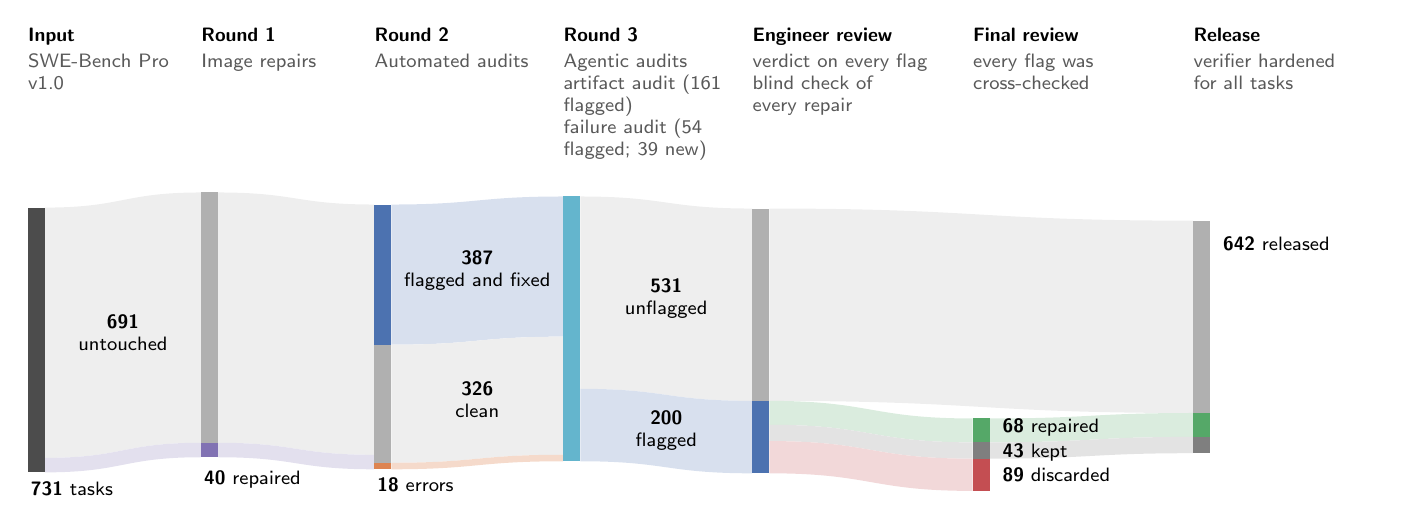
\begin{tikzpicture}[x=1mm, y=1mm, font=\sffamily\scriptsize,
  execute at begin node={\hyphenpenalty=10000\exhyphenpenalty=10000}]
% ---------------------------------------------------------------- bands
% Input -> Round 1: untouched / image repairs
\fill[sbpNone!22] (2.2,-1.92) .. controls (12.1,-1.92) and (12.1,0) .. (22,0)
  -- (22,-31.786) .. controls (12.1,-31.786) and (12.1,-33.706) .. (2.2,-33.706) -- cycle;
\fill[sbpImg!22] (2.2,-33.706) .. controls (12.1,-33.706) and (12.1,-31.786) .. (22,-31.786)
  -- (22,-33.626) .. controls (12.1,-33.626) and (12.1,-35.546) .. (2.2,-35.546) -- cycle;
% Round 1 -> Round 2
\fill[sbpNone!22] (24.2,0) .. controls (34.1,0) and (34.1,-1.53) .. (44,-1.53)
  -- (44,-33.316) .. controls (34.1,-33.316) and (34.1,-31.786) .. (24.2,-31.786) -- cycle;
\fill[sbpImg!22] (24.2,-31.786) .. controls (34.1,-31.786) and (34.1,-33.316) .. (44,-33.316)
  -- (44,-35.156) .. controls (34.1,-35.156) and (34.1,-33.626) .. (24.2,-33.626) -- cycle;
% Round 2 -> Result: flagged / clean / audit errors
\fill[sbpFlag!22] (46.2,-1.53) .. controls (57.1,-1.53) and (57.1,-0.51) .. (68,-0.51)
  -- (68,-18.312) .. controls (57.1,-18.312) and (57.1,-19.332) .. (46.2,-19.332) -- cycle;
\fill[sbpNone!22] (46.2,-19.332) .. controls (57.1,-19.332) and (57.1,-18.312) .. (68,-18.312)
  -- (68,-33.308) .. controls (57.1,-33.308) and (57.1,-34.328) .. (46.2,-34.328) -- cycle;
\fill[sbpErr!30] (46.2,-34.328) .. controls (57.1,-34.328) and (57.1,-33.308) .. (68,-33.308)
  -- (68,-34.136) .. controls (57.1,-34.136) and (57.1,-35.156) .. (46.2,-35.156) -- cycle;
% Result -> Round 3: unflagged / flagged
\fill[sbpNone!22] (70.2,-0.51) .. controls (81.1,-0.51) and (81.1,-2.04) .. (92,-2.04)
  -- (92,-26.466) .. controls (81.1,-26.466) and (81.1,-24.936) .. (70.2,-24.936) -- cycle;
\fill[sbpFlag!22] (70.2,-24.936) .. controls (81.1,-24.936) and (81.1,-26.466) .. (92,-26.466)
  -- (92,-35.666) .. controls (81.1,-35.666) and (81.1,-34.136) .. (70.2,-34.136) -- cycle;
% Round 3 -> Release: never flagged, bypasses engineer review
\fill[sbpNone!22] (94.2,-2.04) .. controls (121.1,-2.04) and (121.1,-3.58) .. (148,-3.58)
  -- (148,-28.006) .. controls (121.1,-28.006) and (121.1,-26.466) .. (94.2,-26.466) -- cycle;
% Round 3 -> Engineer review: repaired / kept / discarded
\fill[sbpRep!22] (94.2,-26.466) .. controls (107.1,-26.466) and (107.1,-28.7) .. (120,-28.7)
  -- (120,-31.736) .. controls (107.1,-31.736) and (107.1,-29.502) .. (94.2,-29.502) -- cycle;
\fill[sbpKeep!22] (94.2,-29.502) .. controls (107.1,-29.502) and (107.1,-31.736) .. (120,-31.736)
  -- (120,-33.806) .. controls (107.1,-33.806) and (107.1,-31.572) .. (94.2,-31.572) -- cycle;
\fill[sbpDisc!22] (94.2,-31.572) .. controls (107.1,-31.572) and (107.1,-33.806) .. (120,-33.806)
  -- (120,-37.9) .. controls (107.1,-37.9) and (107.1,-35.666) .. (94.2,-35.666) -- cycle;
% Engineer review -> Release
\fill[sbpRep!22] (122.2,-28.7) .. controls (135.1,-28.7) and (135.1,-28.006) .. (148,-28.006)
  -- (148,-31.042) .. controls (135.1,-31.042) and (135.1,-31.736) .. (122.2,-31.736) -- cycle;
\fill[sbpKeep!22] (122.2,-31.736) .. controls (135.1,-31.736) and (135.1,-31.042) .. (148,-31.042)
  -- (148,-33.112) .. controls (135.1,-33.112) and (135.1,-33.806) .. (122.2,-33.806) -- cycle;
% ---------------------------------------------------------------- nodes
\fill[black!70] (0,-35.546) rectangle (2.2,-1.92);
\fill[sbpNone]  (22,-31.786) rectangle (24.2,0);
\fill[sbpImg]   (22,-33.626) rectangle (24.2,-31.786);
\fill[sbpFlag]  (44,-19.332) rectangle (46.2,-1.53);
\fill[sbpNone]  (44,-34.328) rectangle (46.2,-19.332);
\fill[sbpErr]   (44,-35.156) rectangle (46.2,-34.328);
\fill[sbpRes]   (68,-34.136) rectangle (70.2,-0.51);
\fill[sbpNone]  (92,-26.466) rectangle (94.2,-2.04);
\fill[sbpFlag]  (92,-35.666) rectangle (94.2,-26.466);
\fill[sbpRep]   (120,-31.736) rectangle (122.2,-28.7);
\fill[sbpKeep]  (120,-33.806) rectangle (122.2,-31.736);
\fill[sbpDisc]  (120,-37.9) rectangle (122.2,-33.806);
\fill[sbpNone]  (148,-28.006) rectangle (150.2,-3.58);
\fill[sbpRep]   (148,-31.042) rectangle (150.2,-28.006);
\fill[sbpKeep]  (148,-33.112) rectangle (150.2,-31.042);
% ---------------------------------------------------------------- labels
\node[anchor=north west, inner sep=1pt] at (0,-36.3) {\textbf{731} tasks};
\node[align=center] at (12.1,-17.8) {\textbf{691}\\untouched};
\node[anchor=north west, inner sep=1pt] at (22,-35.0) {\textbf{40} repaired};
\node[align=center] at (57.1,-9.9) {\textbf{387}\\flagged and fixed};
\node[align=center] at (57.1,-26.3) {\textbf{326}\\clean};
\node[anchor=north west, inner sep=1pt] at (44,-35.8) {\textbf{18} errors};
\node[align=center] at (81.1,-13.5) {\textbf{531}\\unflagged};
\node[align=center] at (81.1,-30.3) {\textbf{200}\\flagged};
\node[anchor=west, inner sep=1pt] at (123.4,-29.9) {\textbf{68} repaired};
\node[anchor=west, inner sep=1pt] at (123.4,-33.0) {\textbf{43} kept};
\node[anchor=west, inner sep=1pt] at (123.4,-35.9) {\textbf{89} discarded};
\node[anchor=west, inner sep=1pt] at (151.4,-6.5) {\textbf{642} released};
% ---------------------------------------------------------------- stage headers
\node[anchor=north west, inner sep=0pt, text width=20mm, align=left] at (0,21)
  {{\bfseries Input}\\[1.5pt]\textcolor{black!65}{SWE-Bench Pro\\v1.0}};
\node[anchor=north west, inner sep=0pt, text width=20mm, align=left] at (22,21)
  {{\bfseries Round 1}\\[1.5pt]\textcolor{black!65}{Image repairs}};
\node[anchor=north west, inner sep=0pt, text width=22mm, align=left] at (44,21)
  {{\bfseries Round 2}\\[1.5pt]\textcolor{black!65}{Automated audits}};
\node[anchor=north west, inner sep=0pt, text width=22mm, align=left] at (68,21)
  {{\bfseries Round 3}\\[1.5pt]\textcolor{black!65}{Agentic audits\\artifact audit (161 flagged)\\failure audit (54 flagged; 39 new)}};
\node[anchor=north west, inner sep=0pt, text width=26mm, align=left] at (92,21)
  {{\bfseries Engineer review}\\[1.5pt]\textcolor{black!65}{verdict on every flag\\blind check of\\every repair}};
\node[anchor=north west, inner sep=0pt, text width=26mm, align=left] at (120,21)
  {{\bfseries Final review}\\[1.5pt]\textcolor{black!65}{every flag was\\cross-checked}};
\node[anchor=north west, inner sep=0pt, text width=24mm, align=left] at (148,21)
  {{\bfseries Release}\\[1.5pt]\textcolor{black!65}{verifier hardened\\for all tasks}};
\end{tikzpicture}}%
\caption{Flow of the 731 tasks from SWE-Bench Pro v1.0 to the released set;
bar and band heights are proportional to task counts. Round~1 repairs 40
container images (leaked test and fixture files, non-standard instructions).
Round~2's automated audit flags 387 tasks (all fixed by human experts). In Round~3, the artifact audit (an LLM agent and a human
auditor compare the instruction with the tests and reference patch) and the
failure audit (an LLM judge attributes failed runs of four agent setups) flag
200 tasks. Engineers adjudicate every flag, and a repair ships only after a
blind re-implementation of the edited instruction passes the hidden tests.}
\label{fig:pipeline}
\end{figure*}

\subsection{Agentic audits}
\label{sec:audits}

\paragraph{Artifact audit.}
An LLM agent compared each task's instruction with its test lists and reference patch, without executing anything. It flagged six patterns: test requirements missing from the instruction, instruction statements contradicted by the tests, test or solution detail copied into the instruction, changed behaviour that no graded test exercises, fixtures read by the tests but never created, and graded lists naming a whole test file. Overly verbose requirement sections were a leakage signal, as they often transcribed the reference patch. A human auditor reviewed the flags and marked high-priority cases; 161 tasks were flagged.

\paragraph{Failure audit.}
We ran four agent configurations on every task: Claude Code with Claude Opus~5, Codex with GPT-5.6, and mini-SWE-agent with both models. For each run, an LLM judge read the trajectory, patch, verifier log and graded tests and attributed each failure to the model or to the task. A task was flagged when a patch consistent with a reasonable reading of the instruction was rejected. For example, in a \textit{vuls} task two configurations fell back to the bundle directory name as instructed and reported \texttt{Sample.app}, while the graded test expects \texttt{Sample} because the reference patch strips the suffix without the instruction saying so. For each such flag we record the defect type, the fix location, an effort estimate, a proposed edit, and the passing and failing configurations. The failure audit flagged 54 tasks, 39 of them new, for 200 flagged tasks in all.


\subsection{Defect taxonomy}
\label{sec:taxonomy}

We merged the audits' labels and the final review's edit types into the six categories of Table~\ref{tab:repairs-discards}; each task is counted once, under its main edit (instruction, else test patch, else grading files). Unstated requirements, contradictions and verifier or environment defects make correct solutions fail; leakage and insufficient tests make a task easier than intended or let an incomplete solution pass.

\begin{table}[t]
\centering
\small
\setlength{\tabcolsep}{3pt}
\begin{tabularx}{\columnwidth}{@{}>{\raggedright\arraybackslash}p{2.05cm} >{\raggedright\arraybackslash}X r r@{}}
\toprule
\textbf{Category} & \textbf{Description} & \textbf{Rep.} & \textbf{Disc.} \\
\midrule
Solution leakage & The instruction gives away test or solution detail. & 18 & 4 \\
\addlinespace
Spec--test contradiction & The instruction contradicts what the tests check. & 10 & 5 \\
\addlinespace
Unstated test requirement & The tests require behaviour, names or files the instruction never states. & 119 & 22 \\
\addlinespace
Insufficient tests & The tests miss part of the change or check incidental details instead of behaviour. & 1 & 33 \\
\addlinespace
Verifier or environment defect & The grading setup or container decides the score regardless of the solution. & 228 & 19 \\
\addlinespace
Miscellaneous & -- & 15 & 6 \\
\midrule
\textbf{Total} & & \textbf{391} & \textbf{89} \\
\bottomrule
\end{tabularx}
\caption{Defect categories of tasks repaired and kept (Rep.) and discarded (Disc.) between the 731 tasks of SWE-Bench Pro Public v1.0 and the final 642. Together, 480 of the 731 tasks (66\%) were repaired or removed. Each task is counted once, under the defect its main edit addresses. Every task also received the hardened verifier, and no reference solution was changed.}
\label{tab:repairs-discards}
\end{table}

\paragraph{Unstated test requirement (119 repaired, 22 discarded).}
The tests depend on behaviour, names or files the instruction does not mention; the \textit{vuls} task above was repaired by stating that the \texttt{.app} suffix is removed. Most of the 119 repairs (25 from confirmed flags, 94 from the final review) are short additions stating something the graded tests already enforce: an exact value, string, ordering or signature. A task was discarded when the test checks how the reference patch happens to be written, stating that would give the solution away.

\paragraph{Spec--test contradiction (10 repaired, 5 discarded).}
The instruction says one thing and the graded test checks another. Wrong instructions were corrected (8 from flags, 2 in the final review); contradictions whose fix lies in the tests were discarded, for example a \textit{webclients} task whose interface declares an \texttt{Element} argument while the graded test passes a \texttt{Document}.

\paragraph{Solution leakage (18 repaired, 4 discarded).}
Leaky instructions walked through the reference patch file by file, or copied expected values from the tests. A \textit{tutanota} instruction told the agent to update the try-catch block around \texttt{aes256Decrypt} in \texttt{decrypt}; the repaired version specifies behaviour only: a \texttt{CryptoError} raised by the crypto library must surface as the application's own \texttt{CryptoError}, which the credentials layer converts to \texttt{KeyPermanentlyInvalidatedError}. Repairs delete the leaked text and, where a test depends on it, restate the requirement as behaviour. The four discards were repaired and then removed before release (\S\ref{sec:review}).

\paragraph{Insufficient tests (1 repaired, 33 discarded).}
The graded tests leave part of the change unchecked: in a \textit{flipt} task they cover only the error paths of a new cache layer, so a \texttt{getJSON} that always returns false and a no-op \texttt{setJSON} pass. Engineers did not write new tests, so these tasks were discarded; the one repair adds a single assertion to a \textit{teleport} test.

\paragraph{Verifier or environment defect (228 repaired, 19 discarded).}
In 16 discarded tasks the fail-to-pass list names a whole file (e.g.\ \texttt{test/tests/calendar/\allowbreak CalendarUtilsTest.js \textbar{} test suite}), so any unrelated or flaky failure in that file fails a correct patch; in 3 the image prevents grading, for example a \textit{teleport} test skipped because SoftHSM is missing, which the verifier scores as a failure. The 228 repaired tasks are those whose only task-specific change was to grading files (223): run scripts narrowed from the whole repository to the package with the graded tests in the four Go repositories, parsers, and the graded-test names of 20 \textit{element-web} tasks; plus 5 instructions that gained an environment fact such as the absence of network or an exact dependency version. Shared verifier defects were fixed for all tasks (\S\ref{sec:verifier}).

\paragraph{Miscellaneous (15 repaired, 6 discarded).}
Fifteen instructions were reworded or given implementation detail that fixes no defect. The six discarded tasks had no flag that held: two \textit{ansible} tasks were quarantined after a leakage flag was rejected, and four were repaired and dropped although their recorded flag did not hold.


\subsection{Engineer review}
\label{sec:review}

Engineers applied one criteria: if the reference patch adds a behaviour that a hidden test checks, the instruction must state the behaviour, but not how the reference patch implements it. Tests were not edited to agree with an instruction, and instructions were never rewritten to match wrong tests.

23 contracted engineers adjudicated every flag in 404 hours. For each claim they recorded whether it holds, holds in part or does not hold, citing artifact and line (e.g.\ \texttt{test\_patch\_before:178}); high-priority flags received a second independent review and a third pass by the project team. A flag that did not hold left the task unchanged (45 tasks; 26 of these rejected flags claimed solution leakage, the type that most often did not hold). A flag whose gap was in the instruction led to an edit limited to where the flag held (69 tasks, 53 of them in the release). A flag whose remedy lay in the tests, fixtures, verifier or image led to quarantine (73 tasks, mostly insufficient tests, 32, and verifier or environment defects, 19). Engineers corrected 55 tasks in all: 51 for a flag that held in full or in part (18 solution leakage, 8 spec--test contradiction, 25 unstated requirement) and 4 for a flag that a later review rejected, which remain in the release through their other edits. With the final review's edits to flagged tasks, 68 of the 200 flagged tasks carry an edit, 43 are unchanged and 89 were discarded (Figure~\ref{fig:pipeline}).

Repairs were validated blind: a second engineer who had seen neither the original task nor the reference patch implemented the edited instruction, and the edit shipped only if that implementation passed the hidden tests. Sixteen repaired tasks were removed before release; we count them as discards under their original flag, and they include all four leakage discards.

\paragraph{Final review.}
Before release, a final pass cross-checked every flag and reviewed the whole set, making task-specific edits to 340 further tasks: 116 instruction edits, one test patch with an added assertion and grading-file changes on 223 tasks, distributed over the rows of Table~\ref{tab:repairs-discards} as given above. A task counts as repaired in the table if one of its own files changed between v1.0 and the release (instruction, test patch, graded-test list, parser or run script); changes applied identically to every task (\texttt{test.sh}, the Dockerfile, \texttt{task.toml} and the pytest worker pin) are not counted.


\subsection{Verifier hardening}
\label{sec:verifier}

Defects in shared grading code were fixed for all tasks; per-task grading files that changed form the verifier row of Table~\ref{tab:repairs-discards} where they were a task's only change.

\paragraph{Scoping and resources.}
The Go verifier ran \texttt{go test ./...} over the whole repository. Scoping it to the graded packages on 253 tasks removed out-of-memory failures and timeouts. Run scripts on 231 tasks that executed the full suite were restricted to the graded tests. With automatic worker counts, pytest-xdist spawned up to 128 workers on small test files and crashed with ``no tests ran'': we capped it at four workers on 239 tasks and inside \texttt{ansible-test} on 83.

\paragraph{Parsing and environment.}
The jest parser assigned tests in failing files to the wrong file and dropped failures (47 tasks), and it truncated test titles at the first parenthesis: it now strips only the trailing timing. We added kernel headers for cgo builds (5 tasks), fetched at grading time one Go module missing from an image's offline cache, re-derived test scoping on 3 tasks that omitted the packages defining the graded tests, and restored CRLF line endings in a fixture that made the reference patch fail.

\paragraph{Test-file reset.}
Before the hidden tests run, the verifier (i)~restores every path the test patch touches and deletes only paths it creates; (ii)~restores modified tracked test data (test data, fixtures, mocks, snapshots), with allowlists for the six reference patches that change fixtures; (iii)~removes agent-written test files that collide with hidden tests; (iv)~clears stale git lock files left by killed agent commands; and (v)~deletes \texttt{\_\_pycache\_\_} and \texttt{.pyc} files. Without (i), agent edits to snapshots owned by the test patch made it fail to apply in 44 runs. Step (v) addresses \texttt{.pyc} files that an agent's \texttt{git stash} round trip left with unchanged size and timestamp, which made the verifier import the base code.

On the assembled 642-task set, the reference patch passes every task and the empty patch fails every task.


\subsection{Hardened evaluation protocol}
\label{sec:protocol}

We run every model under a \textit{locked protocol} where the harness sets network access per phase of a run, and grades the agent's patch in a fresh container rather than in the agent's sandbox.

\paragraph{Network.}
With the network open, 32 of 642 Claude Opus~5 trajectories contacted code hosts, and 25 downloaded the task's own repository. Under the lock, the sandbox can reach only the model endpoint during the agent phase (the allowlist names that hostname alone), web tools that scaffolds execute outside the sandbox are disabled, and the images carry no fixing commit in their git history.

\paragraph{Grading.}
The original harness ran the verifier in the sandbox the agent had just used. Because the verifier restores test files but not binaries, a scripted agent that edits no source file and replaces \texttt{python3} with a script printing \textsc{PASSED} scores 1. Forged dependencies pass through the same gap: with the network closed, some agents that could not fetch a fix edited the Go module cache in place or served a fabricated module version from a local \texttt{GOPROXY}, and neither change appears in the diff. We now save the agent's changes as a patch, apply it to a fresh copy of the task image, run the unchanged verifier there and report that grade, so that binaries or module caches do not carry over.
%We report both grades for every task. When the two disagree, two more fresh grades decide, by majority.
% CHECK: CHEATING_MODES.md says the fresh re-grade is authoritative and that flips are adjudicated with 2 extra fresh re-grades (a forgery fails 2/2, a flake passes at least 1/2). Align the commented sentence with that before re-enabling it.

\paragraph{Trajectory audits.}
A fresh re-grade cannot catch a forgery committed inside the patch, so we audit patches for \texttt{replace} directives that point into the patch or to absolute paths, \texttt{go.sum} entries for modules absent from the image, and large new directories that imitate a third-party SDK. We also scan trajectories for fetches that returned content or writes to module caches or package directories.
% CHECK: state whether flagged patches are rejected automatically or reviewed by hand.